\documentclass{article}
\usepackage[utf8]{inputenc}
\usepackage[russian]{babel}
\usepackage[T2A]{fontenc}
\usepackage{csquotes}
\usepackage{graphicx}
\usepackage{listings}
\usepackage{listingsutf8}
\usepackage{listingsutf8}
\usepackage{listingsutf8}
\usepackage{listingsutf8}
\usepackage{listingsutf8}
\usepackage{listingsutf8}
\usepackage{listingsutf8}
\usepackage{listingsutf8}
\usepackage{listingsutf8}
\usepackage{listingsutf8}
\usepackage{listingsutf8}
\usepackage{listingsutf8}
\usepackage{listingsutf8}
\lstset{
basicstyle=\ttfamily\footnotesize,
language=Python,
columns=fullflexible,
breaklines=true
}
\usepackage{hyperref}

\begin{document}

\title{Реализация модели распознавания чертежей (CAD2Program) в JAX/Flax}
\author{}
\date{}
\maketitle

\section{Обзор архитектуры модели}

Модель основывается на подходе CAD2Program, предлагающем преобразовывать чертеж в текстовую программу описания геометрии. Архитектура имеет два основных компонента: Vision Transformer (ViT) для кодирования изображения чертежа и трансформер-декодер для генерации текстовой последовательности, описывающей геометрические примитивы и их параметры. Такой подход относится к категории vision-language моделей, объединяющих зрение и язык, подобно мультимодальным моделям (например, GPT-4V, LLaVA и др.).

\paragraph{ViT-энкодер изображения.} Входной чертёж (скан или фото рукописного чертежа) обрабатывается ViT-энкодером, который разбивает изображение на патчи (например, $16\times16$ пикселей) и преобразует их в последовательность эмбеддингов фиксированной размерности. К последовательности патчей добавляется обучаемый класс-токен и позиционные эмбеддинги, после чего она пропускается через несколько слоёв трансформера-энкодера. ViT извлекает из изображения высокоуровневые признаки; в частности, класс-токен (или усреднённое представление патчей) служит интегральным представлением всего чертежа. ViT-модели зарекомендовали себя как эффективные энкодеры изображений в различных задачах компьютерного зрения, и в данном случае позволяют обработать чертёж целиком как растровое изображение, не требуя предварительного выделения векторных элементов или разделения на слои.

\paragraph{Трансформер-декодер (Language Model).} Выход ViT-энкодера поступает в трансформер-декодер, задачей которого является сгенерировать последовательность токенов, описывающих геометрические примитивы и их параметры. В работе CAD2Program в качестве декодера используется большой языковый модель (LLM) InternLM-1.8B, которая получает на вход текстовый промпт и дополнительно мультимодальные эмбеддинги изображения. В нашей реализации можно задействовать аналогичный принцип: декодер авторегрессионно предсказывает текст токен за токеном, на каждом шаге принимая во внимание ранее сгенерированные токены (self-attention) и признаки изображения из энкодера (cross-attention). Таким образом модель порождает описание чертежа в виде \textit{программы}: список примитивов (прямоугольников, окружностей, дуг, полилиний и т.,д.) и соответствующих параметров (координаты, размеры, углы, радиусы и т.,п.).

Важно подчеркнуть, что вывод модели представлен в текстовой форме, что даёт несколько преимуществ. Во-первых, текстовое описание легко расширяется новыми типами примитивов или свойств без изменения структуры модели. Во-вторых, используя текст, модель может выписывать числовые значения параметров практически без потерь точности, избегая ошибок квантования – числа просто копируются из аннотаций чертежа (например, размерных линий) в ответ. В-третьих, языковая модель обладает знанием синтаксиса и может генерировать вывод в формате псевдо-кода или готового к выполнению скрипта (например, на Python, как в CAD2Program). Такой vision-language подход позволяет модели одновременно анализировать визуальные элементы чертежа (геометрию и текстовые аннотации) и формировать семантически богатое описание в человекочитаемой форме.

\begin{figure}[h!]
\centering
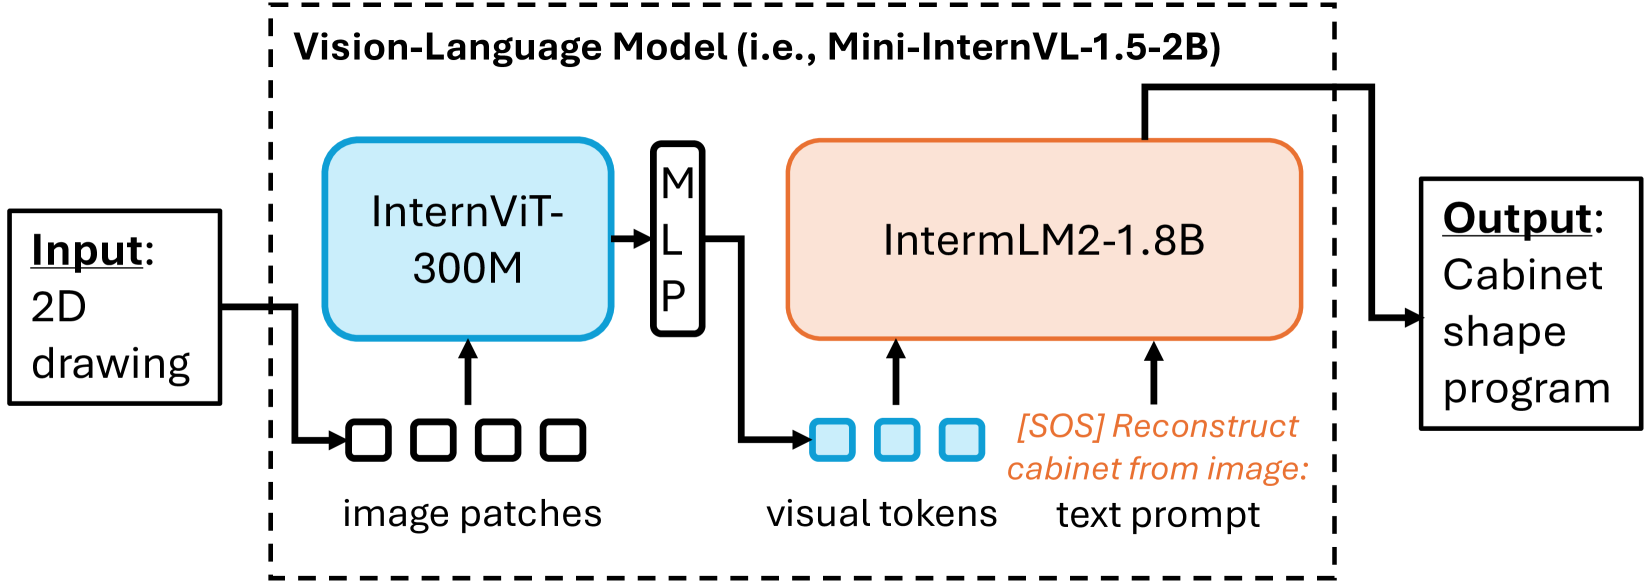
\includegraphics[width=0.95\textwidth]{internvl.png}
\caption{Обзор архитектуры модели CAD2Program: ViT-энкодер (InternViT) извлекает признаки из изображения чертежа, проекция MLP сопоставляет их со скрытым пространством декодера, и языковая модель (InternLM) генерирует текстовую программу примитивов.}
\end{figure}

На \textbf{рисунке 1} показана схема такой архитектуры, соответствующая модели CAD2Program. Для мультимодальной интеграции используется небольшой полносвязный проектор (MLP), который преобразует выход энкодера в формат, пригодный для подачи в языковую модель. В оригинале CAD2Program в декодер подавалась текстовая подсказка "\texttt{Reconstruct cabinet from image:}" перед основным выводом, однако в нашем случае можно использовать более простой промпт (либо специальный токен начала последовательности). В ходе генерации декодер комбинирует визуальный контекст (эмбеддинги изображения) и собственно историю генерируемых токенов, последовательно порождая список примитивов с параметрами.

Подход vision-language обоснован тем, что 2D-чертёж содержит как геометрическую, так и текстовую информацию (размеры, обозначения). Ранее многие методы 3D-реконструкции игнорировали аннотации и работали только с геометрией, требуя предварительного отделения надписей. Наша модель же учится напрямую "читать" чертёж во всём его многообразии, извлекая размеры и другие пометки из изображения. Это стало возможным благодаря использованию крупной предобученной языковой модели, способной понимать текст и цифры, а также благодаря обучению на большом датасете, включающем разнообразные чертежи с их описаниями. В результате модель достигает точности, сравнимой с методами, работающими по векторному CAD-входу, хотя оперирует только растровым изображением.

\section{Пошаговая реализация модели в JAX/Flax}

Далее приведена реализация описанной модели с использованием JAX/Flax. Мы рассмотрим подготовку данных, создание архитектуры энкодера и декодера, процесс обучения модели и осуществление инференса для новых изображений. Код будет приведён на языке Python с использованием библиотеки Flax (в которой реализованы основные компоненты нейросетей для JAX).

\subsection{Подготовка данных}

Для обучения модели необходим набор пар {\textit{чертёж, описание-программа}}. В идеальном случае можно собрать реальный датасет технических чертежей с аннотациями. Если таковой недоступен, прибегают к синтетическому генератору данных. Например, \textbf{Free2CAD} генерирует случайные эскизы объектов и соответствующие скрипты CAD-команд для них. По аналогии, можно автоматически создавать изображения примитивов с проставленными размерными линиями: случайным образом размещать прямоугольники, окружности и другие фигуры, добавлять к ним текстовые обозначения (длины, радиусы), после чего рендерить полученный чертёж в картинку. Одновременно генерируется и целевая текстовая последовательность: перечень примитивов и их параметров, совпадающих с изображением.

При наличии реальных данных (например, сканов чертежей) может понадобиться предварительная разметка: вручную или полуавтоматически описать каждый чертёж набором примитивов. Однако подход CAD2Program предполагает, что модель научится сама выделять примитивы и читать их размеры, поэтому явный разметчик может не потребоваться – достаточно иметь готовые соответствия изображений и параметров, из которых можно сформировать текст программы.

Изображения чертежей конвертируются в тензоры (например, numpy- или JAX-массивы) фиксированного размера. Обычно применяется приведение к масштабу (например, $224\times224$ пикселей) и нормализация значений пикселей. Текстовые описания (программы) токенизируются – разбиваются на токены согласно словарю. Можно использовать либо готовый токенайзер языковой модели (если декодер основан на предобученном LLM), либо специализированный токенайзер, учитывающий формат описания (например, разделяющий имена примитивов и числа). В простейшем случае каждый символ можно считать отдельным токеном, однако эффективнее применить byte-pair encoding или SentencePiece для кодирования строк параметров. На выходе подготовки данных мы получаем набор обучающих примеров вида:
$$X_i = \text{image}_i,\qquad Y_i = [t_1, t_2, \dots, t_{N_i}],$$
где $Y_i$ – последовательность целевых токенов для чертежа $i$.

Для последующего использования в JAX данные часто упаковываются в \texttt{tf.data.Dataset} или в формат TFRecord, но можно работать и с обычными numpy-массивами, разрезая их на батчи. Главное – организовать эффективное чтение и аугментации (например, случайные повороты или добавление шума к изображениям, чтобы повысить устойчивость модели к рукописным вариациям).

\subsection{Архитектура модели на Flax}

Мы определяем два основных модуля Flax: \texttt{VisionEncoder} для ViT-энкодера и \texttt{TextDecoder} для авторегрессорного декодера. Ниже приведён упрощённый код реализации этих модулей.

\begin{lstlisting}
import jax.numpy as jnp
from flax import linen as nn

# Vision Transformer Encoder

class VisionEncoder(nn.Module):
    embed_dim: int = 768
    patch_size: int = 16
    num_layers: int = 12
    num_heads: int = 12

    def setup(self):
        # Проекция патча и класс-токен
        self.patch_embed = nn.Dense(self.embed_dim)
        self.cls_token = self.param('cls_token', nn.initializers.normal(stddev=0.02), (1, 1, self.embed_dim))
        self.pos_embedding = self.param('pos_embedding', nn.initializers.normal(stddev=0.02),
                                        (1, (image_size//self.patch_size)**2 + 1, self.embed_dim))
        # Transformer Encoder layers
        self.transformer_layers = [nn.SelfAttention(num_heads=self.num_heads) for _ in range(self.num_layers)]
        self.mlp_layers = [nn.Sequential([
                                  nn.Dense(self.embed_dim*4), nn.gelu, nn.Dense(self.embed_dim)
                              ]) for _ in range(self.num_layers)]
        self.norm = nn.LayerNorm()

    def __call__(self, img):
        # img shape: (H, W, 3)
        patches = extract_patches(img, patch_size=self.patch_size)  # пользовательская функция
        tokens = self.patch_embed(patches)  # shape: (num_patches, embed_dim)
        # prepend CLS token
        cls = jnp.tile(self.cls_token, (tokens.shape[0], 1, 1))    # (batch, 1, embed_dim)
        x = jnp.concatenate([cls, tokens], axis=1) + self.pos_embedding  # добавляем позиционные эмбеддинги
        # Transformer encoder
        for sa, mlp in zip(self.transformer_layers, self.mlp_layers):
            # Multi-head self-attention block
            x = x + sa(x)              # residual connection
            x = x + mlp(x)            # MLP block with residual
        encoded = self.norm(x)        # shape: (batch, 1+num_patches, embed_dim)
        return encoded
\end{lstlisting}

В приведённом коде энкодера мы опустили детали функции \texttt{extract_patches}, которая разбивает изображение на патчи и выстраивает их в последовательность (размерность \texttt{num_patches} = $(H/\texttt{patch_size})\times(W/\texttt{patch_size})$). После проекции патчей линейным слоем и добавления обучаемого \texttt{[CLS]}-токена, выполняются $L$ слоёв трансформера: каждый слой включает многоголовый self-attention и последующий MLP (полносвязный слой с активацией GELU и выходной проекцией), оба с residual-коннектами и слоём нормализации (LayerNorm). Выход \texttt{encoded} имеет размерность $(B, N_p+1, D)$, где $B$ – размер батча, $N_p$ – число патчей, $D$ – размер эмбеддинга. Для передачи декодеру обычно используется либо весь набор эмбеддингов патчей, либо только эмбеддинг класс-токена (как обобщённое представление изображения). В CAD2Program, например, использовался весь набор визуальных токенов (разбитого на тайлы изображения).

Теперь определим декодер. В упрощённом варианте это авторегрессивный трансформер, который на каждом шаге генерирует следующий токен, имея доступ к предыдущим токенам (через self-attention) и к закодированному изображению (через cross-attention). Мы можем использовать стандартный трансформер-декодер из Flax, но для демонстрации напишем схему вручную:

\begin{lstlisting}
# Transformer Decoder with cross-attention

class TextDecoder(nn.Module):
    vocab_size: int
    embed_dim: int = 768
    num_layers: int = 12
    num_heads: int = 12

    def setup(self):
        # Token embedding and positional embedding
        self.token_embed = nn.Embed(self.vocab_size, self.embed_dim)
        self.pos_embedding = self.param('dec_pos_embedding', nn.initializers.normal(stddev=0.02),
                                        (1, max_seq_len, self.embed_dim))
        # Transformer Decoder layers
        self.self_attn_layers = [nn.SelfAttention(num_heads=self.num_heads) for _ in range(self.num_layers)]
        self.cross_attn_layers = [nn.MultiHeadDotProductAttention(num_heads=self.num_heads) for _ in range(self.num_layers)]
        self.mlp_layers = [nn.Sequential([
                                  nn.Dense(self.embed_dim*4), nn.gelu, nn.Dense(self.embed_dim)
                              ]) for _ in range(self.num_layers)]
        self.norm = nn.LayerNorm()
        # Final language modeling head
        self.output_proj = nn.Dense(self.vocab_size)

    def __call__(self, encoded_image, input_tokens):
        # encoded_image: (batch, N_enc, D), input_tokens: (batch, T)
        x = self.token_embed(input_tokens) + self.pos_embedding[:, :input_tokens.shape[1], :]
        # Masked self-attention to prevent looking ahead
        attn_mask = nn.make_causal_mask(input_tokens)  # triangle causal mask
        for sa, ca, mlp in zip(self.self_attn_layers, self.cross_attn_layers, self.mlp_layers):
            x = x + sa(x, mask=attn_mask)              # self-attention (causal)
            x = x + ca(query=x, key=encoded_image, value=encoded_image)  # cross-attention
            x = x + mlp(x) 
        x = self.norm(x)
        logits = self.output_proj(x)  # shape: (batch, T, vocab_size)
        return logits
\end{lstlisting}

Здесь \texttt{nn.MultiHeadDotProductAttention} – модуль Flax, реализующий механизм внимания “запрос-ключ-значение” между двумя последовательностями (то есть используется для cross-attention с ключами/значениями из энкодера и запросами из декодера). Мы используем causal mask (\texttt{make_causal_mask}) для self-attention, чтобы декодер не видел будущие токены последовательности. На выходе декодера получаются \textit{логиты} размерности $(B, T, V)$, где $T$ – длина последовательности, $V$ – размер словаря. Для получения вероятностей применяется softmax по размерности $V$. В процессе обучения мы будем сравнивать эти логиты с истинной последовательностью токенов.

Наконец, объединим энкодер и декодер в одну модель для удобства тренировки:

\begin{lstlisting}
class CADModel(nn.Module):
    vocab_size: int
    # Параметры encoder/decoder опущены для краткости
    
    def setup(self):
        self.encoder = VisionEncoder()
        self.decoder = TextDecoder(vocab_size=self.vocab_size)
    
    def call(self, image, input_tokens):
        enc = self.encoder(image)  # (B, N_enc, D)
        logits = self.decoder(encoded_image=enc, input_tokens=input_tokens)
        return logits
\end{lstlisting}

Заметим, что для обучения авторегрессии декодер получает в \texttt{input_tokens} правильную последовательность, сдвинутую на один шаг (Teacher Forcing): например, \texttt{input_tokens} = $[\langle \text{BOS}\rangle, t_1, t_2, \dots, t_{N-1}]$, а целевые токены для расчёта лосса = $[t_1, t_2, \dots, t_{N-1}, t_N, \langle \text{EOS}\rangle]$. Таким образом, на $i$-ом шаге декодер видит все предыдущие правильные токены и учится предсказывать следующий $t_i$.

При инициализации модели можно использовать предобученные веса: например, инициализировать \texttt{VisionEncoder} из модели ViT, обученной на ImageNet, и \texttt{TextDecoder} из предобученной языковой модели (с соответствующей загрузкой эмбеддингов и слоёв трансформера). В случае кадров CAD2Program были использованы готовые веса InternViT и InternLM, что значительно ускорило обучение и повысило качество. В нашей реализации для простоты мы можем начать обучение "с нуля" или загрузить близкую по архитектуре модель (например, ViT-B/16 и какой-либо GPT-2/T5 для декодера) и затем дообучить её на нашей задаче.

\subsection{Обучение модели}

Обучение проводится с минимизацией функции потерь cross-entropy между предсказанными и истинными токенами программы. После каждого шага декодера имеем распределение $\hat{y}_i$ по словарю, и вычисляем $-\sum_i y_{i}\log \hat{y}_i$, где $y_i$ – one-hot представление правильного токена на данном шаге. Лосс усредняется по всем токенам последовательности и по батчу:
$$L(\theta) = - \frac{1}{B}\frac{1}{T}\sum_{b=1}^B \sum_{t=1}^{T} \log P_\theta(y_{b,t} \mid x_b, y_{b,<t}),$$
где $x_b$ – изображение, $y_{b,<t}$ – уже сгенерированные токены до шага $t$ (teacher forcing обеспечивает, что это реальные токены на этапе обучения).

В JAX для обучения мы компилируем функцию потерь и её градиент. Используем Optax (библиотека оптимизаторов для JAX) для определения оптимизатора, например AdamW. Ниже показан набросок цикла обучения:

\begin{lstlisting}
import optax
from flax.training import train_state

# Создаём объект модели и начальное состояние параметров

model = CADModel(vocab_size=len(vocab))
rng = jax.random.PRNGKey(0)
params = model.init(rng, jnp.zeros((1, image_size, image_size, 3)),
                    jnp.zeros((1, max_len), dtype=jnp.int32))['params']

# Определяем состояние обучения

tx = optax.adamw(learning_rate=1e-4)
state = train_state.TrainState.create(apply_fn=model.apply, params=params, tx=tx)

@jax.jit
def train_step(state, batch):
    """Выполняет шаг обучения на одном батче данных."""
    def loss_fn(params):
        logits = model.apply({'params': params}, batch['image'], batch['input_tokens'])
        # считаем cross-entropy лосс
        labels = batch['target_tokens']  # ожидаемые токены (shape: [B, T])
        loss = optax.softmax_cross_entropy_with_integer_labels(logits, labels).mean()
        return loss
    # вычисляем значение функции потерь и градиенты
    loss, grads = jax.value_and_grad(loss_fn)(state.params)
    # обновляем параметры
    new_state = state.apply_gradients(grads=grads)
    return new_state, loss

# Итеративное обучение

for epoch in range(num_epochs):
    for batch in data_loader:
        state, loss = train_step(state, batch)
        print(f"Epoch {epoch}: loss = {loss}")
\end{lstlisting}

В этом коде \texttt{train_state} – удобная оболочка от Flax, хранящая параметры и оптимизатор. Функция \texttt{train_step} помечена \texttt{@jax.jit} для компиляции и запуска на GPU/TPU, что значительно ускоряет тренинг. Внутри мы вычисляем градиенты loss-функции с помощью \texttt{jax.value_and_grad}. Используется \texttt{optax.softmax_cross_entropy_with_integer_labels}, которая принимает логиты и целевые индексы токенов, возвращая вектор потерь для каждого элемента, после чего мы берём среднее. Градиенты применяются через \texttt{state.apply_gradients}, которое внутри выполнит шаг оптимизатора (AdamW).

Стоит отметить, что обучение полной модели с нуля – ресурсоёмкий процесс. В оригинальной работе CAD2Program обучение проводилось на 64 GPU (RTX 4090) около суток для датасета из $\sim$368k чертежей. В наших условиях объёмы могут быть меньше, но всё же для сходимости может потребоваться десятки эпох по большим батчам. Предобучение энкодера/декодера сокращает необходимое время тренировки.

\subsection{Инференс (генерация описания)}

После обучения (или в процессе валидации) необходимо реализовать инференс: получение последовательности примитивов по входному изображению. Здесь модель работает в авторегрессионном режиме генерации. Можно воспользоваться стандартными методами генерации текста, применяемыми для языковых моделей – например, жадный поиск (greedy decoding) или поиск с лучом (beam search). Для простоты опишем greedy-подход:
\begin{enumerate}
\item Получаем эмбеддинги изображения через энкодер: $h = \text{encoder}(image)$.
\item Инициализируем последовательность вывода стартовым токеном (например, \texttt{<BOS>} или просто пустой контекст).
\item Передаем текущую последовательность токенов в декодер и получаем логиты для следующего токена.
\item Выбираем токен с максимальной вероятностью (аргмакс по логитам последнего шага) и добавляем его к последовательности.
\item Если токен оказался токеном конца последовательности (\texttt{<EOS>}) или достигнута максимальная допустимая длина, останавливаем генерацию. Иначе возвращаемся к шагу 3.
\end{enumerate}

Ниже приведён псевдокод (на Python) для функции генерации:

\begin{lstlisting}
def generate_primitives(params, image, max_len=100):
    enc = model.encoder.apply({'params': params['encoder']}, image)
    tokens = [vocab['<BOS>']]
    for t in range(max_len):
        logits = model.decoder.apply({'params': params['decoder']}, enc, jnp.array([tokens], dtype=jnp.int32))
        next_token = int(jnp.argmax(logits[0, -1]))
        if next_token == vocab['<EOS>']:
            break
        tokens.append(next_token)
    return [vocab.id_to_token[t] for t in tokens[1:]]
\end{lstlisting}

Эта функция (предполагая, что \texttt{params} разделён на подсловарь для энкодера и декодера) возвращает список сгенерированных токенов (без начального BOS). По этим токенам затем можно восстановить структуру примитивов. Например, если выходные токены образуют строку \texttt{"rectangle(x=10,y=15,w=40,h=20); circle(x=30,y=5,r=5)"}, нужно спарсить её в необходимые параметры или напрямую интерпретировать как команды. В CAD2Program выход формировался в виде синтаксически корректного Python-кода с присвоениями переменных, который можно исполнять для получения 3D-модели. В нашем случае достаточно получить структуру данных – список словарей или объектов, например:
$$[ \{\text{type}: \text{"rectangle"}, x:10, y:15, w:40, h:20\}, \{\text{type}:\text{"circle"}, x:30, y:5, r:5\} ].$$

Чтобы повысить надёжность инференса, можно применять beam search (храня несколько наиболее вероятных последовательностей и расширяя их) или добавить к жадной выборке температурное сэмплирование, штраф повторов и другие приёмы из области NLP. Впрочем, задача детерминирована аннотациями на чертеже, поэтому жадный поиск обычно достаточен – модель должна однозначно вывести правильные цифры и типы примитивов.

\section{Интеграция с ClearML}

Для удобства экспериментов и отслеживания метрик мы интегрируем процесс обучения и инференса с платформой ClearML. ClearML обеспечивает автоматическое логирование параметров и результатов, хранение моделей и простой деплой через ClearML-Serving. Ниже рассмотрены основные шаги интеграции.

\subsection{Логирование экспериментов и метрик}

Интеграция начинается с инициализации задачи эксперимента в ClearML. В коде это делается командой:
\begin{lstlisting}
from clearml import Task
task = Task.init(project_name=“CADPrimitives”, task_name=“Train CAD2Program model”)
\end{lstlisting}
После этого запущенный скрипт связывается с ClearML-сервером (локальным или облачным). ClearML автоматически собирает информацию о среде, параметрах запуска и даже об используемых моделях.

Гиперпараметры (например, размеры слоёв, скорость обучения, размер батча) можно логировать через \texttt{task.connect}, чтобы они отобразились в интерфейсе:
\begin{lstlisting}
config = {"embed_dim": 768, "num_layers": 12, "lr": 1e-4, "batch_size": 32}
task.connect(config)
\end{lstlisting}
Это сохранит словарь параметров эксперимента.

Во время обучения мы можем отправлять в ClearML значения метрик. ClearML автоматически подхватывает стандартные метрики из популярных фреймворков, но в случае ручной тренировки на JAX стоит явно использовать \texttt{Logger}:
\begin{lstlisting}
from clearml import Logger
logger = task.get_logger()

for epoch in range(num_epochs):
    for batch in data_loader:
        state, loss = train_step(state, batch)
    # Логируем ошибку после каждой эпохи
    logger.report_scalar("loss", "train", epoch, float(loss))
\end{lstlisting}
Команда \texttt{report_scalar} фиксирует скалярное значение (например, \texttt{loss}=0.024) в текущей итерации (эпохе). В веб-интерфейсе ClearML эти точки отобразятся на графике. Аналогично можно логировать метрики точности, время шага, или произвольные данные. Например, возможно логировать примеры сгенерированных описаний для валидационного набора, используя \texttt{logger.report_text} или добавлять изображения чертежей с наложенными распознанными примитивами через \texttt{report_image}.

ClearML также сохраняет stdout/стderr вашего скрипта, что упрощает отладку. В итоге каждый запуск тренировки будет задокументирован: какой код и параметры использовались, какие метрики получены, какие артефакты сохранены. Это обеспечивает воспроизводимость экспериментов и удобное сравнение разных запусков модели.

\subsection{Сохранение моделей и чекпоинтов}

После (или в ходе) обучения необходимо сохранить веса модели. Поскольку Flax хранит параметры в виде immutable-диктов, их можно сериализовать с помощью \texttt{flax.serialization.to_bytes} или \texttt{pickle}. Например:
\begin{lstlisting}
import os, pickle

# Сериализуем параметры

weights_bytes = flax.serialization.to_bytes(state.params)
with open("model_ckpt.pkl", "wb") as f:
    f.write(weights_bytes)
\end{lstlisting}
Этот файл \texttt{model_ckpt.pkl} содержит состояние обученной модели. Мы можем сохранять чекпоинты периодически (например, каждые $N$ итераций) для защиты от сбоев и для возможности отката к лучшей версии (по метрике).

ClearML предоставляет удобный способ хранения таких моделей: \textbf{OutputModel}. Мы можем либо вручную загрузить файл как артефакт эксперимента, либо использовать метод \texttt{Task.update_output_model}. Один из простых способов:
\begin{lstlisting}
from clearml import OutputModel
OutputModel.update_checkpoint(task=task,
                              iteration=num_epochs,
                              path="model_ckpt.pkl",
                              name="CAD2Program_model")
\end{lstlisting}
Эта команда загрузит файл \texttt{model_ckpt.pkl} в хранилище ClearML (например, на ClearML Server или облачное хранилище) и присвоит ему имя. После этого в интерфейсе эксперименту будет соответствовать \emph{модель}, которую можно скачать или сразу задеплоить.

Альтернативно, можно вызвать \texttt{task.upload_artifact(“model_final”, “model_ckpt.pkl”)}, тогда файл окажется привязан как артефакт. Разница в том, что \texttt{OutputModel} регистрирует конкретно модель и ее метаданные, и её проще потом использовать с ClearML-Serving.

\paragraph{Деплой через ClearML-Serving.} После того, как модель зарегистрирована, мы можем развернуть её с помощью ClearML-Serving для удаленного инференса. ClearML-Serving состоит из сервиса (контроллера) и одного или нескольких рабочих процессов-инференсов, которые можно запускать в Docker-контейнерах. Взаимодействие происходит через CLI \texttt{clearml-serving}. Основные шаги деплоя:
\begin{enumerate}
\item Запуск сервиса Serving: создаём новую служебную задачу-сервис в ClearML (например, через веб-интерфейс или CLI). Она получит свой идентификатор (Service ID). Для примера пусть \texttt{service_id = SERV1234}.
\item Регистрация модели в сервисе: выполняем команду CLI на машине, где установлен \texttt{clearml-serving}:
\begin{verbatim}
$ clearml-serving --id SERV1234 model add \
    --engine "python" \
    --endpoint "cad_model" \
    --model-id "<ID модели в репозитории>" \
    --preprocess "preprocess.py" \
    --postprocess "postprocess.py"
\end{verbatim}
Параметр \texttt{--model-id} указывает на уникальный ID модели, сохраненной в ClearML (его можно скопировать из UI, или ClearML напечатает его при регистрации модели). \texttt{--engine "python"} означает, что мы сами определим, как выполнять инференс (в отличие от, скажем, \texttt{--engine torchserve} или \texttt{triton} для стандартных фреймворков). Это гибкий режим, где мы можем задать произвольный Python-препроцессинг и постпроцессинг. Файлы \texttt{preprocess.py} и \texttt{postprocess.py} – скрипты, которые будут выполняться перед подачей запроса модели и после получения ответа. В них мы опишем, как преобразовать входное изображение (например, прочитать байты изображения из HTTP-запроса, превратить в тензор нужной формы, возможно, выполнить аугментации) и как обработать выход модели (например, список токенов преобразовать в удобный JSON с примитивами). Эти скрипты тоже будут упакованы ClearML-Serving и храниться на сервере.
\item Запуск inferencing контейнера: ClearML-Serving позволяет запускать инференс как Docker-контейнер. Для этого достаточно выполнить:
\begin{verbatim}
$ docker run -d -p 8080:8080 -e CLEARML_SERVING_TASK_ID=SERV1234 \
    -e CLEARML_SERVING_POLL_FREQ=5 clearml-serving-inference:latest
\end{verbatim}
Здесь мы предполагаем, что образ \texttt{clearml-serving-inference:latest} уже собран (если нет, его можно собрать из репозитория ClearML-Serving). Переменная \texttt{CLEARML_SERVING_TASK_ID} указывает контейнеру, какой сервис (с каким ID) он обслуживает, а \texttt{POLL_FREQ} – как часто проверять обновления. После запуска контейнер подключится к ClearML Server, загрузит зарегистрированную модель и будет готов принимать запросы.
\item Вызов инференса: По умолчанию контейнер слушает порт 8080. ClearML-Serving создает REST API для каждого \texttt{endpoint}. Мы указали \texttt{--endpoint "cad_model"}, значит URL будет \verb|http://localhost:8080/serve/cad_model|. Отправив HTTP POST запрос на этот адрес с входными данными, мы получим ответ модели. Например, можно сделать:
\begin{lstlisting}[language=Python]
import requests, base64
img_bytes = open("test_drawing.png", "rb").read()

# Для передачи изображения в JSON, закодируем его в base64

payload = {"data": base64.b64encode(img_bytes).decode("utf-8")}
res = requests.post("http://localhost:8080/serve/cad_model", json=payload)
print(res.json())
\end{lstlisting}
В \texttt{preprocess.py} должно быть описано, как из JSON извлекается \texttt{data}, декодируется изображение и подготавливается тензор. Аналогично, \texttt{postprocess.py} должен формировать \texttt{res.json()} – например, список примитивов. Результатом запроса будет, например:
\begin{verbatim}
{
  "primitives": [
    {"type": "rectangle", "x": 10, "y": 15, "width": 40, "height": 20},
    {"type": "circle", "x": 30, "y": 5, "radius": 5}
  ]
}
\end{verbatim}
что соответствует распознанным объектам на чертеже.
\end{enumerate}

ClearML-Serving отслеживает версии модели: если, например, переобучить модель и \texttt{publish} её в ClearML, сервис может автоматически обновить деплой до новой версии (эту опцию можно настроить через \texttt{model auto-update}). Также ClearML-Serving предоставляет мониторинг: статистика запросов, время отклика, логирование ошибок – всё это доступно через веб-интерфейс ClearML (раздел \textit{Serving}).

Таким образом, с помощью ClearML мы получаем полный цикл MLOps: отслеживание эксперимента при обучении, хранение и версионирование модели, и развёртывание REST API сервиса для инференса без ручного написания серверного кода. Стоит подчеркнуть, что интеграция потребовала минимальных изменений в коде: по сути, мы добавили несколько вызовов \texttt{Task.init} и \texttt{logger.report}, а деплой осуществляется вообще без изменения основного тренировочного кода.

\section{Деплой модели с помощью vLLM}

Для сценариев, требующих высокой производительности инференса, особенно на больших языковых моделях, удобен инструмент \textbf{vLLM} – специальный движок для ускоренного выполнения LLM-запросов с использованием техники PagedAttention. Хотя наша модель относительно компактна по сравнению с гигантскими GPT-моделями, интеграция с vLLM может дать выигрыш, если требуется обрабатывать множество запросов параллельно (например, сервис распознавания чертежей под высокой нагрузкой). Рассмотрим, как можно задействовать vLLM.

vLLM обеспечивает два основных способа использования:
\begin{enumerate}
\item \textbf{HTTP-сервер, совместимый с OpenAI API.} vLLM может быть запущен как сервер, реализующий REST API, аналогичный эндпоинтам OpenAI (включая \texttt{/v1/completions} и \texttt{/v1/chat/completions}). Это позволяет существующим приложениям, написанным под OpenAI, легко переключиться на локальную модель.
\item \textbf{Библиотека для локального использования.} vLLM предоставляет Python-интерфейс (\texttt{vllm.LLM}), через который можно загружать модель и вызывать генерацию напрямую из кода, без HTTP слоя.
\end{enumerate}

Чтобы использовать vLLM, нашу обученную модель нужно представить в формате, понятном этому движку. vLLM поддерживает модели из Hugging Face Hub или локальные модели в формате Transformers (например, GPT-неподобные архитектуры: GPT-2, GPT-Neo, LLaMA, T5 и др.). Если наш декодер изначально был взят из такой модели (например, мы использовали Mini-InternLM с HuggingFace), то проблем нет – просто указываем путь к модели. Однако, если модель кастомная, может потребоваться написать адаптер или скрипт конвертации весов. Для простоты предположим, что мы fine-tuned версию некого GPT-моделя и сохранили её с помощью \texttt{transformers.FlaxGPT2LMHeadModel}, так что доступен стандартный весовой файл и конфиг.

\paragraph{Запуск vLLM сервера.} Установив \texttt{vllm} (\texttt{pip install vllm}), можно запустить сервер командой:
\begin{verbatim}
$ python -m vllm.entrypoints.openai.api_server \
    --model huggyhub/cad-prim-model \
    --port 8000 --host 0.0.0.0
\end{verbatim}
Здесь вместо \texttt{huggyhub/cad-prim-model} нужно указать либо название модели в HuggingFace Hub, либо локальный путь. После запуска он будет ждать REST запросы на порту 8000, понимая такие же JSON, как OpenAI. Пример запроса (используя Python \texttt{requests}):
\begin{lstlisting}[language=Python]
endpoint = "http://localhost:8000/v1/completions"
prompt = "Extract primitives from drawing: "  # наш промпт, если требуется
payload = {
    "model": "cad-prim-model",
    "prompt": prompt + "<image_embedding>",
    "max_tokens": 100
}
res = requests.post(endpoint, json=payload).json()
print(res["choices"][0]["text"])
\end{lstlisting}
Правда, тут есть нюанс: vLLM в режиме OpenAI API не знает про картинки. Подача изображения возможна, если наша модель оформлена как мультимодальная (например, как в LLaVA, где изображение закодировано специальными токенами). В случае CAD2Program делалось следующее: изображение разбивалось на 12 частей, каждая прогонялась через ViT, и полученные эмбеддинги превращались MLP-проектором в 12 специальных визуальных токенов, добавляемых в начало текстового контекста. Чтобы воспроизвести это с vLLM, можно предварительно вычислить эмбеддинги ViT энкодера в нашем приложении (например, через Flax), затем вставить их как \emph{prefix} в LLM. Однако OpenAI-протокол не поддерживает прямую передачу эмбеддингов. Варианты решения:
\begin{itemize}
\item Запустить vLLM \textbf{в библиотечном режиме} и интегрировать собственный код обработки изображения. Например:
\begin{lstlisting}
from vllm import LLM, SamplingParams
llm = LLM(model="huggyhub/cad-prim-model")
image = load_image("test.png")
image_embeds = vision_encoder.apply(params_enc, image[None, ...])
prompt = "..."  # текстовый промпт, если нужен

# Предположим, модель распознает токен <IMAGE> как сигнал ожидания эмбеддингов

# Добавляем визуальные токены (просто конкатенация признаков) в контекст LLM:

outputs = llm.generate([prompt], image_embeddings=image_embeds, 
                      sampling_params=SamplingParams(max_tokens=100))
print(outputs[0].outputs[0].text)
\end{lstlisting}
Здесь мы воспользовались условно существующим параметром \texttt{image_embeddings} (в действительности vLLM сейчас не предоставляет явного API для мультимодальных токенов, поэтому это псевдокод). В этом случае мы полностью контролируем подачу изображения и можем совместить Flax-энкодер с vLLM-декодером в одной программе. Однако придётся вручную модифицировать архитектуру модели под vLLM.
\item Другой путь – \textbf{расширить REST API} дополнительным эндпоинтом, который принимает изображение. Мы могли бы написать небольшой сервер на базе FastAPI, который внутри вызовет \texttt{llm.generate()} с предварительной обработкой изображения. Впрочем, это уже выходит за рамки возможностей vLLM “из коробки” и представляет кастомное решение.
\end{itemize}

В контексте нашей задачи, возможно, целесообразнее не усложнять и считать, что модель можно разворачивать на vLLM, если она представлена как единая языковая модель, способная по текстовому запросу (включающему описание изображения) выдать ответ. Например, если бы мы обучили модель отвечать на текст вида: "\texttt{На изображении прямоугольник 40x20 и окружность радиуса 5. Примитивы:}" – то она могла бы работать без непосредственной передачи визуальных токенов, а используя распознанные OCR и прочее. Однако тогда теряется суть визуального анализа. Таким образом, прямое применение vLLM требует, чтобы и энкодер, и декодер были слиты в одну модель (как, например, Mini-InternVL, где ViT и LLM объединены). Если мы используем ту же архитектуру, что CAD2Program, можно попытаться экспортировать всю модель (ViT+LLM) в формат, совместимый с HuggingFace Transformers, и затем загрузить в vLLM.

Тем не менее, даже без мультимодального режима, vLLM ценен возможностью динамически батчировать запросы. Если, скажем, у нас есть только декодер (LLM) и мы можем параллельно обрабатывать сразу несколько изображений, vLLM обеспечит групповое выполнение self-attention, уменьшая простои GPU. PagedAttention позволяет гибко управлять памятью KV-кэша, что особенно эффективно при длинных выходных последовательностях. Например, если одна сцена чертежа требует сгенерировать 200 токенов, а другая – 50, обычный батчинг страдал бы от padding или последовательной обработки; PagedAttention хранит состояния запросов и обслуживает их одновременно, устраняя накладные расходы от разной длины.

Подводя итог, интеграция с vLLM может быть реализована следующим образом:
\begin{enumerate}
\item Если модель приведена к формату LLM (без отдельного энкодера), то запустить vLLM-сервер и направлять на него запросы через OpenAI-compatible API, либо
\item Использовать \texttt{vllm.LLM} внутри своего сервиса, реализовав обёртку, которая сама вычисляет визуальные эмбеддинги и передаёт их в модель.
\end{enumerate}
Второй вариант более сложен и потребует модификации vLLM (который заточен под текстовые модели). Поэтому предпочтительнее первый: можно в ClearML-Serving (в скрипте \texttt{preprocess.py}) обращаться к развернутому vLLM-серверу. То есть, ClearML-Serving на себя возьмёт получение изображения, преобразование в текстовый промпт (например, с помощью какой-то OCR или шаблона), отправку на vLLM (который развернул модель, объединяющую знания изображения и текста), и выдачу ответа. Однако это несколько громоздко.

На практике, если требуется одновременно высокая производительность и поддержка визуальных данных, возможно стоит рассмотреть специализированные оптимизации под ViT-энкодер (например, компиляция его через XLA) и сам декодер (тут vLLM не сильно разгонит небольшой 200М параметров модель, ощутимый выигрыш он даёт на миллиардах параметров). Тем не менее, если мы решим увеличить масштаб языкового модуля (скажем, использовать 7B или 13B LLM для большей точности интерпретации чертежей), то развёртывание через vLLM-сервер будет оправдано: он даст 2–4-кратный рост пропускной способности по сравнению с наивным подходом, при той же латентности.

Резюмируя: vLLM можно использовать как высокопроизводительный сервер генерации, совместимый с OpenAI API. Мы подаем ему текстовый запрос, содержащий описание задачи и (опционально) результаты предварительного анализа изображения, и получаем текст программы примитивов. Благодаря оптимальному управлению памятью и агрессивному батчингу запросов, такой сервер сможет обрабатывать множество параллельных запросов распознавания чертежей в реальном времени. Это особенно актуально, если сервис должен масштабироваться на большое число пользователей.

\section{Датасеты и генерация данных}

Качество модели сильно зависит от данных, на которых она обучена. В распоряжении сообщества уже имеются как открытые реальные датасеты чертежей, так и методы генерации синтетических наборов. Мы рассмотрим несколько рекомендаций по данным для нашей задачи.

\paragraph{Открытые датасеты технических чертежей.} Одним из примеров является \textbf{DeepCAD} или аналогичные сборники, содержащие пары "чертёж–параметрическая модель". Свежие исследования предоставляют крупные наборы данных: например, в работе CAD2Program собран датасет из 368 тысяч чертежей шкафов с их 3D моделями. К сожалению, он может быть закрытым корпоративным. Однако существуют и публичные: \textbf{Text2CAD Dataset} содержит технические чертежи с описанием на естественном языке, \textbf{ArchCAD-400K} – корпус архитектурных чертежей с аннотацией символов. Также стоит обратить внимание на наборы по распознаванию символов и схем (например, чертежи электрических схем), которые по структуре близки к нашим (несколько слоёв графики и текста). Если задача сфокусирована на простых примитивах (прямоугольники, окружности), можно использовать набор изображений с известными фигурами, например, генерированные графические сцены или аугментированные эскизы.

Перед использованием открытого набора важно убедиться, что формат аннотаций подходит. Например, ArchCAD-400K помечает отдельные условные обозначения (двери, окна и т.п.) и примитивы линий, но не даёт прямого списка примитивов с размерами. В таком случае наш генеративный подход можно адаптировать: модель будет выводить не список команд, а, скажем, JSON-структуру с найденными объектами и их свойствами. По сути, никаких ограничений – всё определяется тем, какие тексты мы хотим, чтобы модель генерировала. Поэтому если данные размечены иначе, можно переформулировать задачу. Но чаще проще создать синтетический набор точь-в-точь под нужный формат вывода.

\paragraph{Синтетические данные.} Генерация синтетических чертежей – мощный инструмент, позволяющий собрать практически неограниченный обучающий датасет. Он особенно полезен для начального обучения модели, после чего можно тонко настроить (fine-tune) модель на небольшом количестве реальных чертежей, чтобы она адаптировалась к стилю рисовки и возможным особенностям (шумы скана, почерк и т.д.).

Для генерации можно использовать как простые программные методы (например, используя Python-библиотеки \texttt{matplotlib}, \texttt{PIL} или \texttt{OpenCV} для отрисовки фигур на изображении), так и специализированные CAD-библиотеки. Например, \textbf{FreeCAD}, \textbf{CADQuery} или \textbf{OpenSCAD} могут программно создавать чертежи: задавая примитивы, получить их 2D проекции, добавить аннотации. Кроме того, есть инструменты для генерации псевдо-рукописных изображений: чтобы имитировать почерк, можно рендерить текстовые аннотации шрифтом, похожим на рукописный, или применять искажения к компьютерному шрифту.

Процесс генерации может выглядеть так:
\begin{enumerate}
\item Задаём случайные параметры сцены: сколько примитивов, каких типов, их параметры (например, генерируем $n$ прямоугольников со случайными сторонами, $m$ окружностей со случайными радиусами, и т.д.). Следим, чтобы примитивы не слишком перекрывались или, наоборот, не были слишком разрежены, стараясь охватить разнообразные конфигурации.
\item Создаём изображение: рисуем оси или сетку (опционально), рисуем каждый примитив. Для прямоугольников и др. можно добавить штриховку или вспомогательные линии, но базово – просто контуры.
\item Для каждого примитива добавляем размерные линии и надписи. Например, для прямоугольника рисуем стрелки от его сторон и рядом текст с числовым значением длины (случайное целое или с десятичной точкой). Для углов – можем добавить дугу и указать величину угла. Здесь важно соблюдать стандарт оформления: размерные линии параллельны измеряемому элементу, имеют выносные линии, а текст обычно пишется по центру над линией. Можно упростить и просто писать число рядом.
\item Получаем итоговое изображение (можно сохранять в PNG).
\item Формируем описание – например, строку: \texttt{"rectangle(x=..., y=..., width=..., height=...); circle(x=..., y=..., r=...)"}. Все значения берем те, что использовали при генерации (которые по сути совпадают с нарисованными на картинке).
\item Повторяем тысячи раз для генерации набора. Включаем разные шрифты для текста, добавляем случайные шумы (небольшое размытие, имитация сканированных документов, фон) для робастности.
\end{enumerate}

Получив такой синтетический набор, его можно сразу использовать для обучения модели с нуля. Опыт показывает, что модель способна обобщать и на реальные данные, если синтетика достаточно разнообразна. Тем не менее, рекомендуется \textit{fine-tuning} на небольшом реально размеченном наборе: это подправит модель, например, научит распознавать реальные почеркушки цифр или нестандартные обозначения, которые сложно предусмотреть программно.

В качестве открытого источника для генерации можно упомянуть \textbf{sketch-rnn dataset} или \textbf{QuickDraw}, где есть много эскизов – но они без размерных аннотаций. Тем не менее, оттуда можно почерпнуть идеи для аугментаций или формы примитивов (хотя QuickDraw – более художественные рисунки).

Если требуется распознавать более сложные объекты (например, условные обозначения или сочетания простых примитивов, образующие фигуры), можно дополнить синтетические данные: либо вручную добавлять такие сложные случаи, либо комбинировать примитивы по правилам. Например, рисовать стрелки, рамки, отрезки – чтобы модель не путала их с границами объекта.

\paragraph{Дополнительное дообучение (fine-tuning).} После базового обучения на синтетике имеет смысл дообучить модель на любых доступных реальных примерах. Даже несколько десятков образцов, близких к целевым данным, могут значительно улучшить качество, особенно в аспектах стилевых отличий. Fine-tuning в Flax аналогичен основной тренировке, только с меньшим learning rate и на небольшое число шагов. Можно воспользоваться уже настроенным \texttt{TrainState}, просто продолжив тренировать на новом датасете, или загрузить сохранённую модель и запустить новый \texttt{train_step} цикл.

При дообучении важно также валидировать модель: в идеале иметь validation set и контролировать, чтобы не произошло переобучения на новых данных. ClearML опять же помогает отслеживать метрики при fine-tuning – можно создать новую задачу в том же проекте, а можно продолжить в старой (тогда ClearML зафиксирует параметр \texttt{task.started_again}).

Наконец, стоит упомянуть, что текущее решение – сначала синтетика, потом реал – соответствует \textit{domain adaptation}. Если разница между синтетикой и реальностью существенная, могут помочь приемы вроде domain randomization (сильно варьировать синтетические данные, чтобы охватить реальный домен) илиGAN-based подходы для перевода изображений синтетики в стиль реальных сканов.

В любом случае, комбинируя открытые наборы и синтетически сгенерированные, разработчик получает полный контроль над обучением. В отличие от чисто rule-based систем, здесь глубокая модель может действительно выучить соответствие пикселей и геометрических параметров, даже в условиях зашумленности или несовершенства входных данных.

\section*{Заключение}

В данном документе мы подробно рассмотрели реализацию модели распознавания геометрических примитивов на чертеже с использованием современных подходов vision-language. Архитектура CAD2Program (ViT-энкодер + трансформер-декодер) доказала свою эффективность для восстановления 3D-моделей по 2D-чертежам, и её идеи успешно применимы для извлечения плоских примитивов с аннотациями. Мы описали, как реализовать такую модель на JAX/Flax, включая ключевые этапы подготовки данных, обучения и инференса, снабдив описание примерами кода. Далее, были рассмотрены вопросы MLOps: интеграция с ClearML для экспериментов и деплоя, а также использование vLLM для ускорения инференса. Наконец, мы обсудили стратегию работы с данными – от генерации большого синтетического датасета до использования открытых наборов и последующего тонкого дообучения.

Следуя изложенным шагам, можно получить работающую систему, которая по загруженному скану рукописного чертежа вернёт список обнаруженных примитивов и их размеров. Такая система найдёт применение в CAD-пакетах для оцифровки старых бумажных чертежей, в образовательных приложениях для разбора геометрических рисунков, либо как вспомогательный инструмент для ускорения 3D-моделирования по эскизам. При дальнейших улучшениях – увеличении данных, использовании более мощных языковых моделей – точность и универсальность подхода будут расти. Уже сейчас, опираясь на накопленные успехи VLM-моделей, наш подход позволяет объединить визуальное восприятие и способность работать с текстом (числами и кодом) в единое решение, существенно упростив задачу, которая ранее решалась раздельно методами компьютерного зрения и алгоритмического анализа чертежей.

\begin{thebibliography}{99}

\bibitem{CAD2Program} Wang, Xilin, et al. \textit{From 2D CAD Drawings to 3D Parametric Models: A Vision-Language Approach}. AAAI, 2025  .

\bibitem{Dosovitskiy2021ViT} Dosovitskiy, Alexey, et al. \textit{An Image is Worth 16x16 Words: Transformers for Image Recognition at Scale}. ICLR, 2021 .

\bibitem{Kwon2023PagedAttn} Kwon, Woosuk, et al. \textit{Efficient Memory Management for Large Language Model Serving with PagedAttention}. SOSP, 2023  .

\bibitem{JAX2018} Bradbury, James, et al. \textit{JAX: composable transformations of Python+NumPy programs}. 2018  .

\bibitem{Flax2020} Heek, Jonathan, et al. \textit{Flax: A neural network library and ecosystem for JAX}. 2020 (version 0.11.2, 2024) .

\bibitem{ClearML} ClearML. \textit{Open-Source MLOps Platform for ML Workflow Management}. \url{https://clear.ml}, accessed 2025  .

\bibitem{Free2CAD2022} Li, Changjian, et al. \textit{Free2CAD: Parsing Freehand Drawings into CAD Commands}. ACM TOG 41(4): 141:1–16, 2022  .

\end{thebibliography}

\end{document}